\section{Триггеры}
\textbf{Формулировка задания.}

Создать таблицу, в которой с помощью триггеров для каждой коровы
поддерживаются актуальные значения количества лактаций и назначенных рационов питания.

\subsection{Создание таблицы}
\textbf{Текстовое объяснение последовательности выполнения команды создания таблицы.}

При выполнении команды создается физическая таблица \\\texttt{Cow\_lactation\_diet\_count}.
В структуре таблицы определяются три поля целочисленного типа (\texttt{INT}):
первичный ключ \texttt{id\_Cow} для идентификации коровы,
а также столбцы \texttt{Lactation\_count} и \texttt{Diet\_count},
предназначенные для хранения актуальных значений количества лактаций и рационов
каждой коровы.

SQL-код создания таблицы \texttt{Cow\_lactation\_diet\_count} приведен в листинге
\ref{lst:Cow_lactation_diet_count}.

\begin{lstlisting}[caption={Создание таблицы Cow\_lactation\_diet\_count}, label={lst:Cow_lactation_diet_count}]
CREATE TABLE IF NOT EXISTS Cow_lactation_diet_count (
    id_Cow INT PRIMARY KEY,
    Lactation_count INT,
    Diet_count INT
);
\end{lstlisting}

\textbf{Текстовое объяснение последовательности выполнения команды заполнения таблицы.}

Для заполнения таблицы \texttt{Cow\_lactation\_diet\_count}
используется команда \texttt{INSERT INTO} в сочетании с подзапросом, считывающим выборку 
\texttt{SELECT}.
В подзапросе к таблице \texttt{Cow} последовательно присоединяются таблицы
\texttt{Lactation, Nutrition, Feeding\_plan} и \texttt{Diet} с помощью
левого внешнего соединения (\texttt{LEFT JOIN}).
Данные группируются по ключевому полю \texttt{Cow.id\_Cow},
после чего агрегатная функция \texttt{COUNT} с ключевым словом \texttt{DISTINCT} рассчитывает количество уникальных лактаций и рационов для каждой коровы. Полученные значения вставляются в соответствующие столбцы созданной таблицы.

В листинге \ref{lst:Cow_lactation_diet_count_заполнение}
приведен SQL-код заполнения таблицы \\\texttt{Cow\_lactation\_diet\_count} данными.

\begin{lstlisting}[caption={Заполнение таблицы Cow\_lactation\_diet\_count}, label={lst:Cow_lactation_diet_count_заполнение}]
INSERT INTO Cow_lactation_diet_count (id_Cow, Lactation_count, Diet_count)
SELECT Cow.id_Cow, 
    COUNT(DISTINCT Lactation.id_Lactation), 
    COUNT(DISTINCT Diet.id_Diet)
FROM Cow 
LEFT JOIN Lactation ON Lactation.id_Cow = Cow.id_Cow
LEFT JOIN Nutrition ON Nutrition.id_Cow = Cow.id_Cow
LEFT JOIN Feeding_plan ON Feeding_plan.id_Feeding_plan = Nutrition.id_Feeding_plan
LEFT JOIN Diet ON Diet.id_Diet = Feeding_plan.id_Diet
GROUP BY Cow.id_Cow;
\end{lstlisting}

На рисунке \ref{fig:схема_бд_англ} представлена схема базы данных на английском языке
с добавлением созданной таблицы \texttt{Cow\_lactation\_diet\_count} и указанием триггеров.

\clearpage
\newgeometry{margin=1cm}
\begin{landscape}
    \begin{figure}[p]
        \centering
        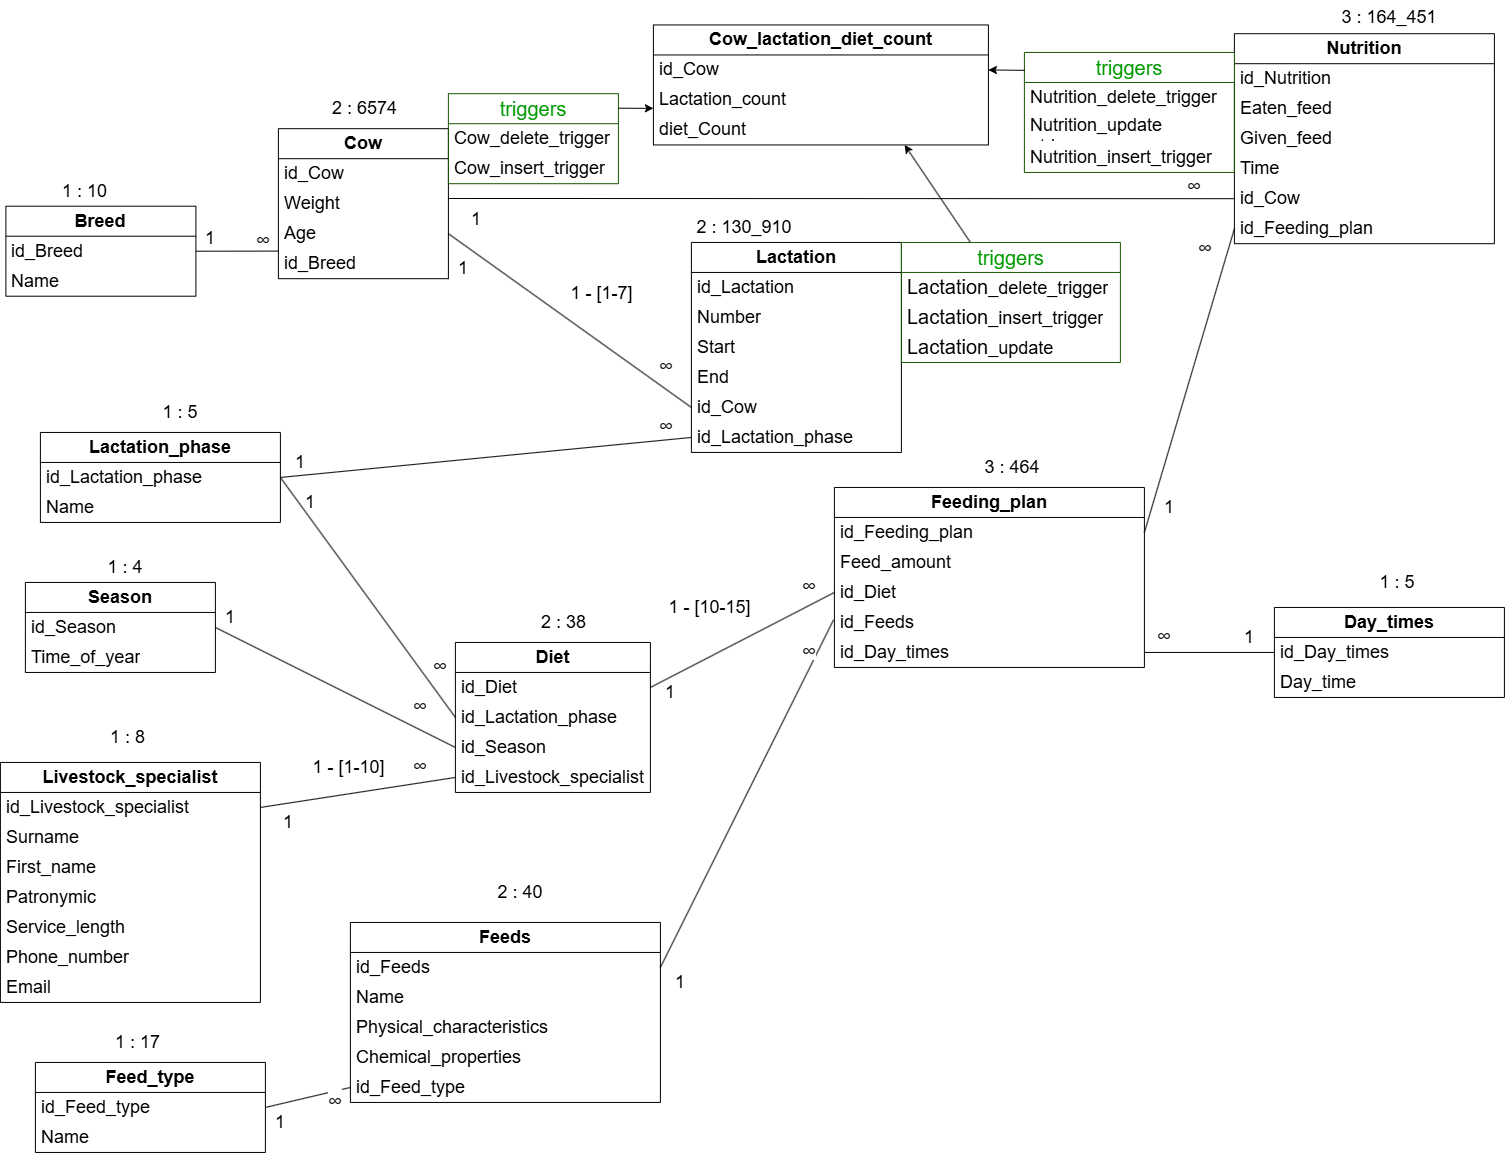
\includegraphics[width=\textwidth, height=\textheight, keepaspectratio]{images/схема_бд_англ_триггеры.png}
        \caption{Схема базы данных на английском языке с триггерами}
        \label{fig:схема_бд_англ}
    \end{figure}
\end{landscape}
\restoregeometry
\clearpage


\subsection{Создание триггеров}

В листинге \ref{lst:Cow_insert_trigger}
приведена SQL-команда создания триггера, срабатывающего после добавления новой записи в таблицу \texttt{Cow}.

\begin{lstlisting}[caption={Создание триггера Cow\_insert\_trigger}, label={lst:Cow_insert_trigger}]
CREATE TRIGGER Cow_insert_trigger
    AFTER INSERT ON Cow 
    FOR EACH ROW EXECUTE FUNCTION Cow_insert_trigger_function();
\end{lstlisting}

В листинге \ref{lst:Cow_insert_trigger_function} представлена SQL-команда создания функции \\
\texttt{Cow\_insert\_trigger\_function}. Функция вызывается триггером \\\texttt{Cow\_insert\_trigger}
и добавляет в таблицу \texttt{Cow\_lactation\_diet\_count} новую запись для зарегистрированной коровы,
инициализируя начальные значения количества лактаций и рационов нулями.
\begin{lstlisting}[caption={Создание функции Cow\_insert\_trigger\_function}, label={lst:Cow_insert_trigger_function}]
CREATE OR REPLACE FUNCTION Cow_insert_trigger_function()
RETURNS TRIGGER AS $$
BEGIN
    INSERT INTO Cow_lactation_diet_count (id_Cow, Lactation_count, Diet_count)
    VALUES (NEW.id_Cow, 0, 0);
    RETURN NEW;
END;
$$ LANGUAGE plpgsql;
\end{lstlisting}

В листинге \ref{lst:Cow_delete_trigger} представлена SQL-команда создания триггера,
срабатывающего после удаления записи из таблицы \texttt{Cow}.

\begin{lstlisting}[caption={Создание триггера Cow\_delete\_trigger}, label={lst:Cow_delete_trigger}]
CREATE TRIGGER Cow_delete_trigger 
    AFTER DELETE ON Cow 
    FOR EACH ROW EXECUTE FUNCTION Cow_delete_trigger_function();
\end{lstlisting}

В листинге \ref{lst:Cow_delete_trigger_function} приведена SQL-команда создания функции \\
\texttt{Cow\_delete\_trigger\_function}.
Функция вызывается триггером \\\texttt{Cow\_delete\_trigger}
и удаляет соответствующую запись из таблицы \texttt{Cow\_lactation\_diet\_count}
по идентификатору удаляемой коровы \\(\texttt{OLD.id\_Cow}).

\begin{lstlisting}[caption={Создание функции Cow\_delete\_trigger\_function}, label={lst:Cow_delete_trigger_function}]
CREATE OR REPLACE FUNCTION Cow_delete_trigger_function()
RETURNS TRIGGER AS $$
BEGIN
    DELETE FROM Cow_lactation_diet_count WHERE id_Cow = OLD.id_Cow;
    RETURN OLD;
END;
$$ LANGUAGE plpgsql;
\end{lstlisting}

В листинге \ref{lst:Nutrition_insert_trigger} представлена SQL-команда создания триггера,
срабатывающего после добавления новой записи в таблицу \texttt{Nutrition}.

\begin{lstlisting}[caption={Создание триггера Nutrition\_insert\_trigger}, label={lst:Nutrition_insert_trigger}]
CREATE TRIGGER Nutrition_insert_trigger
    AFTER INSERT ON Nutrition 
    FOR EACH ROW EXECUTE FUNCTION Nutrition_insert_trigger_function();
\end{lstlisting}

В листинге \ref{lst:Nutrition_insert_trigger_function} приведена SQL-команда создания функции \\
\texttt{Nutrition\_insert\_trigger\_function}.
Функция вызывается триггером \texttt{Nutrition\_insert\_trigger} и выполняет перерасчет количества
уникальных рационов для коровы \texttt{NEW.id\_Cow} (обращение к значению поля id\_Cow из строки,
которая добавлена в таблицу \texttt{Nutrition}) путем объединения таблиц
\texttt{Nutrition, Feeding\_plan} и \texttt{Diet} с помощью \texttt{LEFT JOIN}.
В результате работы функции обновляется значение поля
\texttt{diet\_count} в таблице \texttt{Cow\_lactation\_diet\_count}.

\begin{lstlisting}[caption={Создание функции Nutrition\_insert\_trigger\_function}, label={lst:Nutrition_insert_trigger_function}]
CREATE OR REPLACE FUNCTION Nutrition_insert_trigger_function()
RETURNS TRIGGER AS $$
BEGIN 
    UPDATE Cow_lactation_diet_count 
    SET diet_count = (
        SELECT COUNT(DISTINCT Diet.id_Diet)
        FROM Nutrition
        LEFT JOIN Feeding_plan ON Feeding_plan.id_Feeding_plan = Nutrition.id_Feeding_plan
        LEFT JOIN Diet ON Diet.id_Diet = Feeding_plan.id_Diet
        WHERE Nutrition.id_Cow = NEW.id_Cow
    )
    WHERE id_Cow = NEW.id_Cow; 
    RETURN NEW;
END;
$$ LANGUAGE plpgsql;
\end{lstlisting}

В листинге \ref{lst:Nutrition_delete_trigger} представлена SQL-команда создания триггера,
срабатывающего после удаления записи из таблицы \texttt{Nutrition}.

\begin{lstlisting}[caption={Создание триггера Nutrition\_delete\_trigger}, label={lst:Nutrition_delete_trigger}]
CREATE TRIGGER Nutrition_delete_trigger
    AFTER DELETE ON Nutrition
    FOR EACH ROW EXECUTE FUNCTION Nutrition_delete_trigger_function();
\end{lstlisting}

В листинге \ref{lst:Nutrition_delete_trigger_function} приведена SQL-команда создания функции
\\\texttt{Nutrition\_delete\_trigger\_function}.
Функция вызывается триггером \texttt{Nutrition\_delete\_trigger} и выполняет перерасчет количества
уникальных рационов для коровы \texttt{OLD.id\_Cow} (обращение к значению поля id\_Cow из строки,
которая удалена из таблицы \texttt{Nutrition}) после удаления соответствующей записи.
Результат повторного вычисления обновляет значение столбца \texttt{diet\_count} в таблице
\texttt{Cow\_lactation\_diet\_count}.

\begin{lstlisting}[caption={Создание функции Nutrition\_delete\_trigger\_function}, label={lst:Nutrition_delete_trigger_function}]
CREATE OR REPLACE FUNCTION Nutrition_delete_trigger_function()
RETURNS TRIGGER AS $$
BEGIN
    UPDATE Cow_lactation_diet_count 
    SET diet_count = (
        SELECT COUNT(DISTINCT Diet.id_Diet)
        FROM Nutrition
        LEFT JOIN Feeding_plan ON Feeding_plan.id_Feeding_plan = Nutrition.id_Feeding_plan
        LEFT JOIN Diet ON Diet.id_Diet = Feeding_plan.id_Diet
        WHERE Nutrition.id_Cow = OLD.id_Cow
    )
    WHERE id_Cow = OLD.id_Cow; 
    RETURN OLD;
END;
$$ LANGUAGE plpgsql;
\end{lstlisting}

В листинге \ref{lst:Nutrition_update_trigger} представлена SQL-команда создания триггера,
срабатывающего после обновления записи в таблице \texttt{Nutrition}.
Данная реализация рассчитана на случай изменения только плана кормления.

\begin{lstlisting}[caption={Создание триггера Nutrition\_update\_trigger}, label={lst:Nutrition_update_trigger}]
CREATE TRIGGER Nutrition_update_trigger
    AFTER UPDATE ON Nutrition 
    FOR EACH ROW EXECUTE FUNCTION Nutrition_update_trigger_function();
\end{lstlisting}

В листинге \ref{lst:Nutrition_update_trigger_function} приведена SQL-команда создания функции
\\\texttt{Nutrition\_update\_trigger\_function}.
Функция вызывается триггером \texttt{Nutrition\_update\_trigger} после изменения записи
в таблице \texttt{Nutrition} и выполняет перерасчет количества уникальных рационов для коровы
\texttt{NEW.id\_Cow}, заменяя устаревшее значение в столбце \texttt{diet\_count}
таблицы \texttt{Cow\_lactation\_diet\_count} на актуальное.

\begin{lstlisting}[caption={Создание функции Nutrition\_update\_trigger\_function}, label={lst:Nutrition_update_trigger_function}]
CREATE OR REPLACE FUNCTION Nutrition_update_trigger_function()
RETURNS TRIGGER AS $$
BEGIN
    UPDATE Cow_lactation_diet_count 
    SET diet_count = (
        SELECT COUNT(DISTINCT Diet.id_Diet)
        FROM Nutrition
        LEFT JOIN Feeding_plan ON Feeding_plan.id_Feeding_plan = Nutrition.id_Feeding_plan
        LEFT JOIN Diet ON Diet.id_Diet = Feeding_plan.id_Diet
        WHERE Nutrition.id_Cow = NEW.id_Cow
    )
    WHERE id_Cow = NEW.id_Cow;
    RETURN NEW; 
END;
$$ LANGUAGE plpgsql;
\end{lstlisting}

В листинге \ref{lst:Lactation_insert_trigger} представлена SQL-команда создания триггера,
срабатывающего после добавления новой записи в таблицу \texttt{Lactation}.

\begin{lstlisting}[caption={Создание триггера Lactation\_insert\_trigger}, label={lst:Lactation_insert_trigger}]
CREATE TRIGGER Lactation_insert_trigger
    AFTER INSERT ON Lactation 
    FOR EACH ROW EXECUTE FUNCTION Lactation_insert_trigger_function();
\end{lstlisting}

В листинге \ref{lst:Lactation_insert_trigger_function} приведена SQL-команда создания функции
\\\texttt{Lactation\_insert\_trigger\_function}.
Функция вызывается триггером \texttt{Lactation\_insert\_trigger} при добавлении нового периода лактации
и выполняет перерасчет общего количества лактаций для соответствующей коровы \texttt{NEW.id\_Cow},
обновляя значение столбца \texttt{lactation\_count} в таблице \texttt{Cow\_lactation\_diet\_count}.

\begin{lstlisting}[caption={Создание функции Lactation\_insert\_trigger\_function}, label={lst:Lactation_insert_trigger_function}]
CREATE OR REPLACE FUNCTION Lactation_insert_trigger_function()
RETURNS TRIGGER AS $$
BEGIN
    UPDATE Cow_lactation_diet_count 
    SET lactation_count = 
        (SELECT COUNT(*) FROM Lactation WHERE id_Cow = NEW.id_Cow)
    WHERE id_Cow = NEW.id_Cow;
    RETURN NEW;
END;
$$ LANGUAGE plpgsql;
\end{lstlisting}


В листинге \ref{lst:Lactation_delete_trigger} представлена SQL-команда создания триггера,
срабатывающего после удаления записи из таблицы \texttt{Lactation}.

\begin{lstlisting}[caption={Создание триггера Lactation\_delete\_trigger}, label={lst:Lactation_delete_trigger}]
CREATE TRIGGER Lactation_delete_trigger
    AFTER DELETE ON Lactation
    FOR EACH ROW EXECUTE FUNCTION Lactation_delete_trigger_function();
\end{lstlisting}

В листинге \ref{lst:Lactation_delete_trigger_function} приведена SQL-команда создания функции
\\\texttt{Lactation\_delete\_trigger\_function}.
Функция вызывается триггером \texttt{Lactation\_delete\_trigger} и выполняет
перерасчет количества лактаций для соответствующей коровы \texttt{OLD.id\_Cow},
обновляя значение столбца \texttt{lactation\_count} таблицы \texttt{Cow\_lactation\_diet\_count}.

\begin{lstlisting}[caption={Создание функции Lactation\_delete\_trigger\_function}, label={lst:Lactation_delete_trigger_function}]
CREATE OR REPLACE FUNCTION Lactation_delete_trigger_function()
RETURNS TRIGGER AS $$
BEGIN
    UPDATE Cow_lactation_diet_count 
    SET lactation_count = 
        (SELECT COUNT(*) FROM Lactation WHERE id_Cow = OLD.id_Cow)
    WHERE id_Cow = OLD.id_Cow;  
    RETURN OLD;
END;
$$ LANGUAGE plpgsql;
\end{lstlisting}

В листинге \ref{lst:Lactation_update_trigger} представлена SQL-команда создания триггера,
срабатывающего после обновления записи в таблице \texttt{Lactation}.
Данная реализация не рассчитана на случай изменения \texttt{id\_Cow} коровы.

\begin{lstlisting}[caption={Создание триггера Lactation\_update\_trigger}, label={lst:Lactation_update_trigger}]
CREATE TRIGGER Lactation_update_trigger
    AFTER UPDATE ON Lactation 
    FOR EACH ROW EXECUTE FUNCTION Lactation_update_trigger_function();
\end{lstlisting}

В листинге \ref{lst:Lactation_update_trigger_function} приведена SQL-команда создания функции
\\\texttt{Lactation\_update\_trigger\_function}.
Функция вызывается триггером \texttt{Lactation\_update\_trigger}
и выполняет перерасчет количества лактаций для соответствующей коровы \texttt{NEW.id\_Cow},
обновляя значение столбца \texttt{lactation\_count} в таблице \texttt{Cow\_lactation\_diet\_count}.

\begin{lstlisting}[caption={Создание функции Lactation\_update\_trigger\_function}, label={lst:Lactation_update_trigger_function}]
CREATE OR REPLACE FUNCTION Lactation_update_trigger_function()
RETURNS TRIGGER AS $$
BEGIN
    UPDATE Cow_lactation_diet_count
    SET lactation_count =
        (SELECT COUNT(*) FROM Lactation WHERE id_Cow = NEW.id_Cow)
    WHERE id_Cow = NEW.id_Cow;
    RETURN NEW;
END;
$$ LANGUAGE plpgsql;
\end{lstlisting}

\subsection{Демонстрация работы триггеров}

В таблице \ref{tab:действия_триггеров} представлено описание изменений 
таблицы \\\texttt{Cow\_lactation\_diet\_count} 
посредством триггеров в зависимости от изменения данных в таблицах \texttt{Cow},
\texttt{Nutrition}, \texttt{Lactation}.

\begin{table}[h!]
\centering
\caption{Описание действий триггеров}
\label{tab:действия_триггеров}
\begin{tabular}{|c|p{0.85\textwidth}|}
\hline
\textnumero & {Действие} \\
\hline
1 & Добавление коровы в таблицу \texttt{Cow}. В таблице \texttt{Cow\_lactation\_diet\_count} создаётся запись с нулевыми значениями количества лактаций и рационов. \\
\hline
2 & Удаление коровы из таблицы \texttt{Cow}. Из таблицы \texttt{Cow\_lactation\_diet\_count} удаляется соответствующая запись. \\
\hline
3 & Добавление записи питания в таблицу \texttt{Nutrition}. Пересчитывается количество уникальных рационов для указанной коровы в таблице \texttt{Cow\_lactation\_diet\_count}. \\
\hline
4 & Удаление записи питания из таблицы \texttt{Nutrition}. Пересчитывается количество уникальных рационов для указанной коровы в таблице \texttt{Cow\_lactation\_diet\_count}. \\
\hline
5 & Изменение плана кормления в таблице \texttt{Nutrition}. Пересчитывается количество уникальных рационов для указанной коровы в таблице \texttt{Cow\_lactation\_diet\_count}. \\
\hline
6 & Добавление лактации в таблицу \texttt{Lactation}. Пересчитывается общее количество лактаций для указанной коровы в таблице \texttt{Cow\_lactation\_diet\_count}. \\
\hline
7 & Удаление лактации из таблицы \texttt{Lactation}. Пересчитывается общее количество лактаций для указанной коровы в таблице \texttt{Cow\_lactation\_diet\_count}. \\
\hline
\end{tabular}
\end{table}

На рисунке \ref{cow_insert_example} представлено появление новой записи
в таблице \\\texttt{Cow\_lactation\_diet\_count} после добавления
записи в таблицу \texttt{Cow}.

\begin{figure}[H]
    \centering
    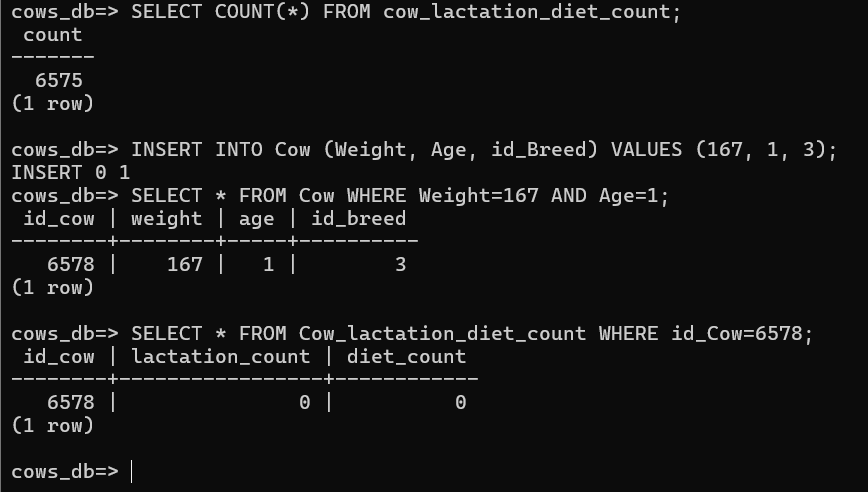
\includegraphics[width=\linewidth]{images/cow_insert_example.png}
    \caption{Результат добавления новой записи в таблицу Cow}
    \label{cow_insert_example}
\end{figure}

На рисунке \ref{delete_cow_example} представлены изменения данных в таблице \\
\texttt{Cow\_lactation\_diet\_count}: отсутствие данных о корове, запись которой
была удалена из таблицы \texttt{Cow}.

\begin{figure}[H]
    \centering
    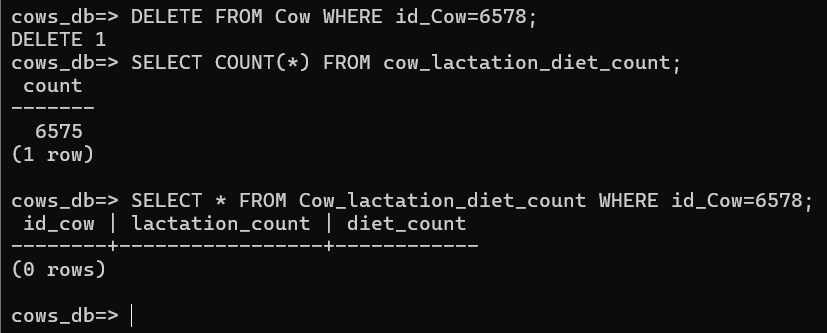
\includegraphics[width=\linewidth]{images/delete_cow_example.png}
    \caption{Результат удаления записи из таблицы Cow}
    \label{delete_cow_example}
\end{figure}

На рисунке \ref{delete_lactation_example} продемонстрировано уменьшение
количества лактаций в таблице
{Cow\_lactation\_diet\_count} после удаления записи в таблице
\texttt{Lactation}.

\begin{figure}[H]
    \centering
    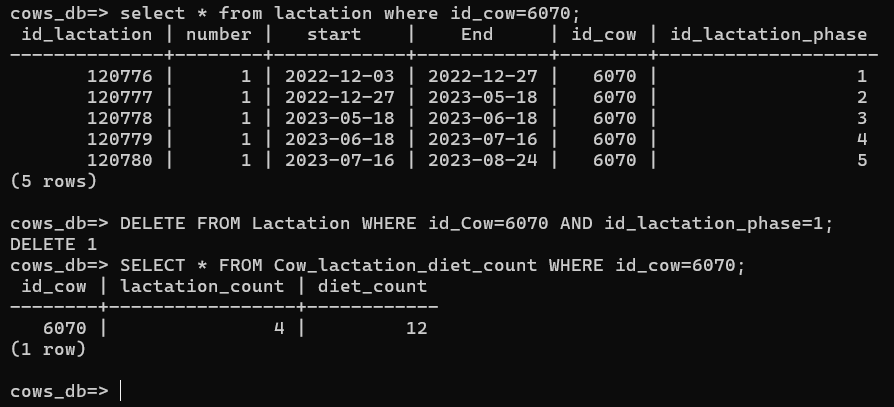
\includegraphics[width=\linewidth]{images/delete_lactation_example.png}
    \caption{Результат удаления записи из таблицы Lactation}
    \label{delete_lactation_example}
\end{figure}

На рисунке \ref{update_nutrition_example} продемонстрировано уменьшение количества
рационов в таблице
\texttt{Cow\_lactation\_diet\_count} после изменения плана кормления
в таблице \texttt{Nutrition}.

\begin{figure}[H]
    \centering
    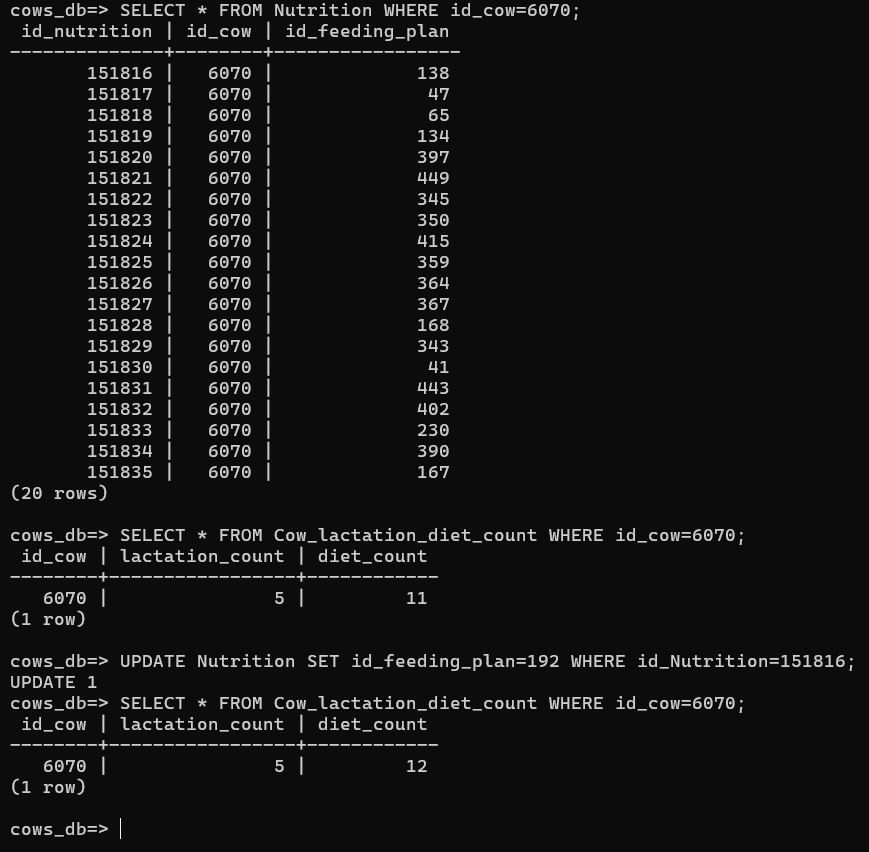
\includegraphics[width=\linewidth]{images/update_nutrition_example.png}
    \caption{Изменение данных при обновлении плана кормления в таблице Nutrition}
    \label{update_nutrition_example}
\end{figure}

